\documentclass[11pt,a4paper]{article}

\usepackage[polish]{babel}
\usepackage[utf8]{inputenc}
\usepackage{polski}
\usepackage[T1]{fontenc}
\usepackage{indentfirst}
\usepackage{wrapfig}    % for wrapping figures, tables

\frenchspacing

%\usepackage{amsmath}
\usepackage{physics}

%\usepackage{bm}
\usepackage{gensymb}
%\usepackage{hepnames}
\usepackage{epsfig}
\usepackage{graphics}
\usepackage[shortlabels]{enumitem}
%\usepackage{xspace}
%\xspaceaddexceptions{[]\{\}}

%
%
%fixpagesize
\pagestyle{empty}
\addtolength{\textwidth}{6cm}
\addtolength{\textheight}{4cm}
\addtolength{\evensidemargin}{-3cm}
\addtolength{\oddsidemargin}{-3cm}
\addtolength{\topmargin}{-3cm}
\parindent=0cm


%
%
%small distance in list/item/enum for enumitem package
\setlist[itemize,enumerate]{topsep=0em}
\setlist{noitemsep}

%print zadanie #
\newcounter{zadanie}\newcommand{\zadanie}[1][]{\addtocounter{zadanie}{1} ~\\  {\bf \emph{Zadanie \arabic{zadanie} #1 }} \\}
\newcounter{zaddom}\newcommand{\zaddom}[1][]{\addtocounter{zaddom}{1} ~\\  {\bf \emph{Zadanie domowe \arabic{zaddom} #1 }} \\}
%\renewcommand{\zadanie}[1][]{\pagebreak  ~\\  {\bf \emph{Zadanie }} \\} \addtolength{\topmargin}{-2cm}


%%%%%%%%%%%%%%%%%%%%%%%%%%%%%%%%%%%%%%%%%%%%%%%%%%%%%%
\begin{document}           % End of preamble and beginning of text.

\begin{centering}
\bf{\Large{Termodynamika z elementami fizyki statystycznej}}\\
Ćwiczenia 1 (1 marca 2021)\\[5mm]
Dochodzenie do równowagi termicznej, rozszerzalność cieplna \\
\end{centering}
\vspace{1mm}

\zadanie
Metalowy blok o temperaturze początkowej $T_1$ umieszczony został
w otoczeniu, którego temperatura przełączana jest regularnie
pomiędzy dwiema ustalonymi wartościami: $T_1$ i $T_2$ ($T_1>T_2$).
Jak zmienia si"e temperatura bloku w funkcji czasu?
Znajdź maksymalną i minimalną temperaturę bloku
w stanie ustalonym (tzn. po bardzo dużej liczbie przełączeń)
i przedyskutuj jako funkcję okresu $b$.
\begin{center}
\resizebox{0.5\linewidth}{!}{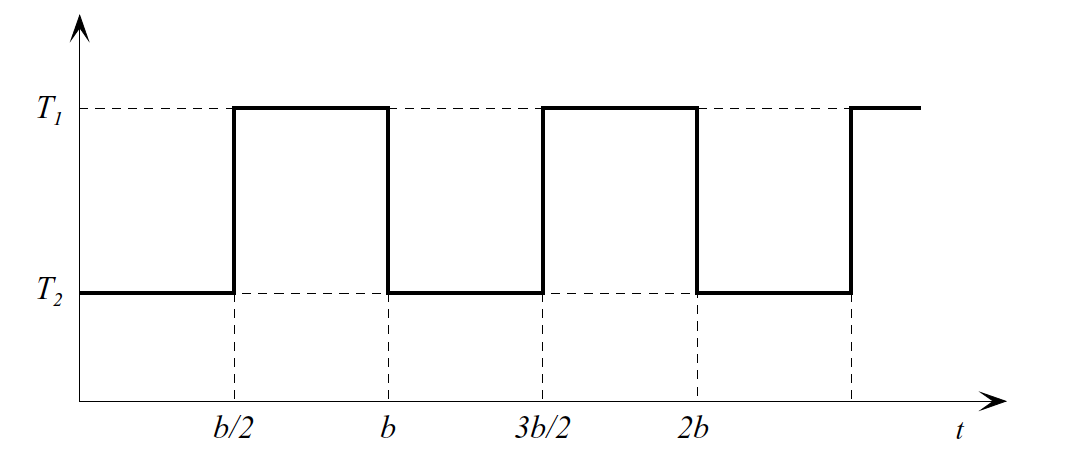
\includegraphics{figure_temp_switching.png}}
\end{center}\vspace{-5mm}
\vskip 10pt
\textbf{Rozwiązanie:}

Stosujemy równanie Newtona
\begin{equation}
	\frac{dT}{dt} = - \alpha (T - T_{\rm ot}).
\end{equation}
W przypadku gdy $T_{\rm ot}$ jest stałe dostajemy
\begin{equation}
	T(t) = A e^{-\alpha t} + T_{\rm ot},
\end{equation}
gdzie $A$ jest stałą którą możemy określić na podstawie warunku początkowego: $A = T(0) - T_{\rm ot}$. Ostatecznie
\begin{equation}
	T(t) = (T(0) - T_{ot})e^{-\alpha t} + T_{\rm ot}. \label{rozwiazanie_Newton}
\end{equation}
Zastosujemy teraz to rozwiązanie dla $T_{\rm ot}$ przełączanej pomiędzy wartościami $T_1$ i $T_2$ zgodnie z wykresem. Załóżmy, że w danej chwili $t$ otoczenie jest w temperaturze $T_2$. To znaczy, że $N b \leq t \leq Nb + b/2$ dla liczby naturalnej $N$. Dodatkowo oznaczmy przez $t'= t - Nb$ czas od ostatniego przełączenia. Zgodnie z wzorem~\eqref{rozwiazanie_Newton} dostajemy
\begin{equation}
	T(t') = (T_{Nb} - T_2) e^{-\alpha t'} + T_2,
\end{equation}
gdzie $T_{Nb}$ jest temperaturą w chwili $Nb$, czyli na początku podcyklu. Na koniec tego podcyklu $t' = b/2$ i temperatura wynosi
\begin{equation}
	T_{Nb + b/2} = (T_{Nb} - T_2) e^{-\alpha b/2} + T_2.
\end{equation}
W tym momencie temperatura otoczenia przełącza się na $T_1$. Oznaczmy przez $t'' = t - (Nb + b/2)$ czas od momentu przełączenia. Ponownie, zgodnie z~\eqref{rozwiazanie_Newton}, otrzymujemy
\begin{equation}
	T(t'') = (T_{Nb +b/2} -T_1) e^{-\alpha t''} + T_1,
\end{equation}
więc na koniec tego podcyklu temperatura wynosi
\begin{equation}
	T_{Nb +b} = (T_{Nb +b/2} -T_1) e^{-\alpha b/2} + T_1.
\end{equation}
Możemy wstawić do tego wzoru $T_{Nb +b/2}$ by otrzymać temperaturę po pełnym cyklu zależną od temperatury na początku tego cyklu. Dostajemy
\begin{equation}
	T_{Nb +b} = \left( (T_{Nb} - T_2)e^{-\alpha b/2} + T_2 - T_1\right) e^{-\alpha b/2} + T_1. \label{jeden_cykl}
\end{equation}
Pytanie o termalizacje: jak informacja o warunkach początkowych ginie w tej sytuacji?

Rozważmy teraz stan ustalony, czyli po dużej liczbie przełączeń. Spodziewamy się, że po dużej liczbie przełączeń, układ po odbyciu pełnego cyklu wraca do temperatury na początku cyklu, czyli
\begin{equation}
	T_{(N+1)b} = T_{Nb}.
\end{equation}
Dostajemy równanie
\begin{equation}
	T_{Nb} = \left( (T_{Nb} - T_2)e^{-\alpha b/2} + T_2 - T_1\right) e^{-\alpha b/2} + T_1.
\end{equation}
Grupując wyrazy z $T_{Nb}$, $T_1$ i $T_2$ dostajemy
\begin{equation}
	T_{Nb}(1 - e^{-\alpha b}) = T_2 \,e^{-\alpha b/2} (1 - e^{-\alpha b/2}) + T_1 (1 - e^{-\alpha b/2})
\end{equation}
i ostatecznie
\begin{equation}
	T_{Nb} = \frac{T_1 + T_2 \,e^{-\alpha b/2}}{1 + e^{-\alpha b/2}}.
\end{equation}
Możemy też łatwo wyznaczyć temperaturę w stanie ustalonym w połowie cyklu. Wstawiając właśnie wyznaczone $T_{Nb}$ do wzoru na $T_{Nb +b/2}$ dostajemy
\begin{equation}
	T_{Nb + b/2} = \frac{T_2 + T_1\, e^{-\alpha b/2}}{1 + e^{-\alpha b/2}}.
\end{equation}
Dostajemy więc, że w stanie ustalonym temperatura zmienia się pomiędzy $T_{\rm min} = T_{Nb +b/2}$ a $T_{\rm max} = T_{Nb}$. Zbadajmy na koniec jak te dwie temperatury zależą od $\alpha$ i $b$. Mamy dwie sytuacje. Gdy $\alpha b \ll 1$ wtedy $T_{\rm min} = T_{\rm max} = (T_1 + T_2)/2$. Natomiast gdy $\alpha b \gg 1$ to $T_{\rm min} = T_2$ a $T_{\rm max} = T_1$. 


Zadanie to możemy też rozwiązać wyznaczając $T_{Nb}$ jako funkcje warunku początkowego. W tym celu policzmy $T_b$, $T_{2b}$ i tak dalej z~\eqref{jeden_cykl}. Dostajemy
\begin{align}
	T_b &= ((T_1 - T_2) e^{-\alpha b/2} + T_2 - T_1)e^{-\alpha b/2} + T_1 = (T_1-T_2)(1 - e^{-\alpha b/2} + e^{-\alpha b}) + T_2, \\
	T_{2b} &= ((T_1 - T_2)(1 - e^{-\alpha b/2} + e^{-\alpha b}) e^{-\alpha b/2} + T_2 - T_1)e^{-\alpha b/2} + T_2 \\
	&= (T_1 - T_2) ( 1 - e^{-\alpha b/2} + e^{-\alpha b} - e^{-3\alpha b/2} + e^{-2\alpha b}) + T_2.
\end{align}
Zgadujemy, że $T_{Nb}$ przyjmuje postać
\begin{equation}
	T_{Nb} = T_2 + (T_1 - T_2) \sum_{j=0}^N q^j,
\end{equation}
gdzie $q = - e^{-\alpha b/2}$. Mamy więc szereg geometryczny który prowadzi do
\begin{equation}
	T_{Nb} = T_2 + (T_1 - T_2) \frac{1 - q^{N}}{1 - q} = T_2 + (T_1 - T_2) \frac{1 + e^{- N \alpha b/2} }{1 + e^{-\alpha b/2}}.
\end{equation}
W granicy dużej liczby przełączeń $N$ jest duże więc możemy zaniedbać ostatni wyraz. Po uporządkowaniu, dostajemy
\begin{equation}
	T_{Nb} = \frac{T_1 + T_2 e^{-\alpha b/2}}{1 + e^{-\alpha b/2}}.
\end{equation}
czyli ten sam wynik co poprzednio.

\zadanie
Blok metalowy umieszczony jest w otoczeniu, którego temperatura
zmienia się według wzoru:
\[T_{ot}(t) = T_\circ + A \cos(\omega t).\]
Początkowa temperatura bloku wynosi $T_\circ$. Znajdź zależność
temperatury bloku od czasu w stanie ustalonym.
\vskip 10pt

\textbf{Rozwiązanie:}
Ponownie korzystamy z równania Newtona
\begin{equation}
	\frac{dT(t)}{dt} = -\alpha (T(t) - T_{\rm ot}(t)).
\end{equation}
Tym razem, temperatura otoczenia zmienia się w czasie. Postulujemy rozwiązanie w postaci
\begin{equation}
	T(t) = C e^{-\alpha t} + K \sin (\omega t) + L \cos (\omega t) + T_0.
\end{equation}
Wstawiając do równania i porównując wyrazy przy $\sin(\omega t)$ i $\cos(\omega t)$ dostajemy dwa równania
\begin{align}
	\alpha (L-A)  &= -\omega K \\
	\alpha K &=  \omega L.
\end{align}
Rozwiązując, znajdujemy
\begin{equation}
	L = \frac{\alpha^2 A}{\omega^2 + \alpha^2}, \qquad K =  \frac{\alpha \omega}{\omega^2 + \alpha^2} A.
\end{equation}
Ostatnią stałą $C$ znajdujemy z warunku początkowego
\begin{equation}
	T_0 = T(0) = C + T_0 + L,
\end{equation}
z czego wynika, że $C = - L$. 

Dla dużych czasów wyraz eksponencjalny możemy zaniedbać więc
\begin{equation}
	T(t) = T_0 + \frac{\alpha A}{\omega^2 + \alpha^2} \left(\omega \sin(\omega t) + \alpha \cos(\omega t)\right).
\end{equation}
Zbadajmy teraz co się dzieje w zależności od $\omega$ i $\alpha$. Gdy $\omega \ll \alpha$ wtedy $T(t) = T_0 + A \cos(\omega t)$. Natomiast gdy $\omega \gg \alpha$ wtedy $T(t) = T_0$.

Rozwiązanie możemy też przedstawic w następującej postaci
\begin{equation}
	T(t) = T_0 + \frac{\alpha A}{\sqrt{\omega^2 + \alpha^2}} \left(\cos \phi \sin(\omega t) + \sin \phi \cos(\omega t)\right) = T_0 + \frac{\alpha A}{\sqrt{\omega^2 + \alpha^2}}\sin(\omega t + \phi),
\end{equation}
gdzie zdefiniowaliśmy
\begin{equation}
	\tan \phi = \frac{\alpha}{\omega}.
\end{equation}


\zadanie
\begin{wrapfigure}{r}{0.3\linewidth}\vspace{-1cm}
\resizebox{\linewidth}{!}{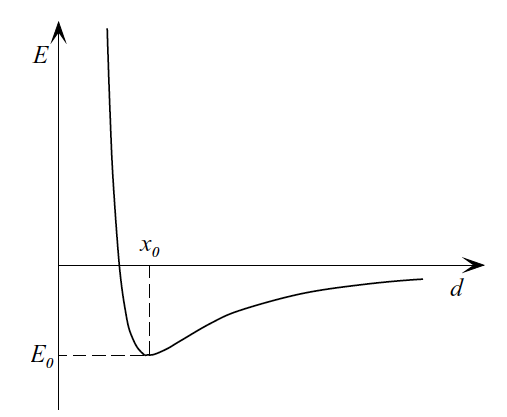
\includegraphics{figure_potencjal.png}}
\end{wrapfigure}
Energia potencjalna oddzia"lywania dw"och atom"ow danej substancji jest
przedstawiona na rysunku obok. Znale"z"c "sredni"a
odleg"lo"s"c mi"edzy atomami odpowiadaj"ac"a energii $E>E_0$,
zak"ladaj"ac, "re:
\begin{enumerate}
\item 
\parbox[t]{\linewidth}{
w pobli"ru punktu r"ownowagi $x=x_0$ energia 
potencjalna daje si"e przybli"ry"c wzorem\\[2mm] 
\centerline{$E_p(x) \approx a (x-x_0)^2 - b (x-x_0)^3 + E_0$,}\\[2mm]
gdzie $a$ i $b$ s"a sta"lymi dodatnimi,
}
\item anharmoniczna poprawka trzeciego rz"edu jest ma"la, tzn. \mbox{$b |x-x_0|\ll a$},
\item punkty zwrotne $x_{\rm min}$ i $x_{\rm max}$
drga"n bardzo niewiele r"o"rni"a si"e od punkt"ow zwrotnych
oscylatora harmonicznego $x^h_{\rm min}$ i $x^h_{\rm max}$ (dla $b=0$),
\item \mbox{średnia odległość międzyatomowa w czasie drgań może być
przybliżona przez średnią} arytmetyczną $\langle x\rangle \approx \frac{x_{\rm min}+x_{\rm max}}{2}$.
\end{enumerate}
\vskip 10pt
\textbf{Rozwiązanie:}

Energia całkowita dwóch atomów składa się z sumy energii potencjalnej i kinetycznej. W punkcie zwrotu energia kinetyczna wynosi zero, więc energia potencjalna jest równa całkowitej energii $E$. Oznaczmy przez $\Delta E = E - E_0$ względną energie układu względem dna studni potencjału. Załóżmy na początek, że potencjał jest harmoniczny. Wtedy
\begin{equation}
	E(x_{\rm min/max}) = a ( x_{\rm min/max}^h - x_0)^2 + E_0,
\end{equation}
lub
\begin{equation}
	\Delta E = a (x_{\rm min/max}^h - x_0)^2.
\end{equation}
Rozwiązując dla $x_{\rm min/max}^h$ dostajemy
\begin{equation}
	x_{\rm min/max}^h = x_0 \mp \sqrt{\frac{\Delta E}{a}},
\end{equation}
i dla średniej odległości międzyatomowej dostajemy $\langle x \rangle = x_0$, czyli odległość nie zależy od energii układu! Zobaczmy co się stanie jak dodamy anharmoniczne poprawki.

Oznaczmy nowe punktu zwrotu przez $x_{\rm min/max}$ i załóżmy, że
\begin{equation}
	x_{\rm min/max} = x_{\rm min/max}^h + \epsilon_{\rm min/max},
\end{equation}
z $\epsilon_{\rm min/max}$ małym. Dostajemy
\begin{equation}
	\Delta E = a ( x_{\rm min/max}^h - x_0 + \epsilon_{\rm min/max})^2 - b ( x_{\rm min/max}^h - x_0 + \epsilon_{\rm min/max})^3.
\end{equation}
Skorzystamy, teraz z faktu, że $\epsilon$ jest małą wielkością. 
\begin{align}
	(x + \epsilon)^2 &= x^2 + 2 x \epsilon + \epsilon^2 = x^2 + 2x \epsilon + \mathcal{O}(\epsilon^2), \\
	(x + \epsilon)^3 &= x^3 + 3 x^2 \epsilon + 3 x \epsilon^2 + \epsilon^3  = x^3 + 3 x^2 \epsilon + \mathcal{O}(\epsilon^2).
\end{align}
Z dokładnością $\epsilon_{\rm min/max}^2$ dostajemy
\begin{equation}
	0 = \mp 2 \sqrt{a \Delta E} \epsilon_{\rm min/max} \pm b \left( \frac{\Delta E}{a}\right)^{3/2} - 3b \sqrt{\frac{\Delta E}{a}} \epsilon_{\rm min/max}.
\end{equation}
Co prowadzi do 
\begin{equation}
	\epsilon_{\rm min/max} = \frac{b \frac{\Delta E}{a}}{2a \pm 3b \sqrt{\frac{\Delta E}{a}}}.
\end{equation}
Wzór ten możemy wciąż trochę uprościć zauważając że, $a \gg b |x - x_0| = b \sqrt{\Delta E/a}$. Prowadzi to ostatecznie do 
\begin{equation}
	\epsilon_{\rm min/max} = \frac{b \Delta E}{2 a^2}, 
\end{equation}
natomiast średnia odległość międzyatomowa wynosi
\begin{equation}
	\langle x \rangle = x_0 + \frac{b \Delta E}{2 a^2}.
\end{equation}
Widzimy, że dzięki anharmoniczności potencjału ($b \neq 0$) średnia odległość między atomami rośnie wraz z ich energią. Ponieważ energia wewnętrzna substancji rośnie wraz z temperaturą, możemy wywnioskować że wraz ze wzrostem temperatury ciała będą się rozszerzać. Jest to zjawisko \emph{rozszerzalności cieplnej}.

\zadanie
Wykaza"c, "re dla materia"lu anizotropowego zachodzi zwi"azek:
$\gamma\,=\,\alpha_1+\alpha_2+\alpha_3$, gdzie $\gamma$ jest wsp"o"lczynnikiem rozszerzalno"sci obj"eto"sciowej danego materia"lu, za"s $\alpha_i ~(i=1,2,3)$
s"a wsp"o"lczynnikami rozszerzalno"sci liniowej wzd"lu"r 3 
nier"ownowa"rnych (i wzajemnie prostopad"lych) kierunk"ow tego materia"lu.

\vskip 10pt

\textbf{Rozwiązanie:} Współczynnik rozszerzalności objętościowej definiujemy zmianę objętości materiału pod wpływem zmiany temperatury podzieloną przez początkową objętość, to znaczy
\begin{equation}
	\gamma = \frac{1}{V} \frac{dV}{dT}.
\end{equation}
W analogiczny sposób możemy zdefiniować współczynniki rozszerzalności liniowej
\begin{equation}
	\alpha_i = \frac{1}{L_i} \frac{d L_i }{dT}.
\end{equation}
Korzystając ze związku $V = L_1 L_2 L_3$ dostajemy
\begin{equation}
	\gamma = \frac{1}{V} \frac{dV}{dT} = \frac{1}{V} \left( L_1 L_2 \frac{d L_3}{dT} + L_3 L_1 \frac{d L_2}{dT} + L_2 L_3 \frac{d L_1}{dT} \right) = \alpha_1 + \alpha_2 + \alpha_3.
\end{equation}

Alternatywnie, współczynniki rozszerzalności mogą być zdefiniowane jako
\begin{equation}
	\gamma = \frac{1}{V_{0}} \frac{dV}{dT}, \qquad \alpha_i = \frac{1}{L_{i, 0}} \frac{d L_i }{dT},
\end{equation} 
gdzie $V_{0}$ i $L_{i, 0}$ są wzorcowymi wymiarami. Wtedy
\begin{equation}
	V \approx V_{0} + \gamma V_{0} \Delta T, \label{aaa}
\end{equation}
oraz 
\begin{equation}
	L_{i} \approx L_{i, 0} + \alpha_{i} L_{i, 0} \Delta T.
\end{equation}
Nowa objętość wynosi więc
\begin{align}
	V &= L_{1} L_{2} L_{3} = L_{1,0} L_{2, 0} L_{3, 0} + (\alpha_{1} + \alpha_{2} + \alpha_{3}) L_{1,0} L_{2, 0} L_{3, 0} \Delta T + A \cdot (\Delta T)^{2} + B \cdot (\Delta T)^{3} \nonumber \\
	&\approx  V_{0} + (\alpha_{1} + \alpha_{2} + \alpha_{3}) V_{0} \Delta T.
\end{align}
Porównując ze wzorem~\eqref{aaa} dostajemy ponownie, że $\gamma = \alpha_{1} + \alpha_{2} + \alpha_{3}$.

\zadanie
Odległość między słupami elektrycznymi wynosi 50\,m.
O ile zmienia swoją długość zawieszony między nimi cienki drut miedziany,
jeżeli temperatura zmienia się od -25\degree C do +35\degree C?
Współczynniki rozszerzalności liniowej miedzi wynosi $\alpha = 8.9\cdot 10^{-6} {\rm K}^{-1}$.
Oszacuj zmianę zwisania drutu.

\vskip 10pt

W przybliżeniu liniowym, długość drutu w temperaturze $T$ zmieni się o
\begin{equation}
	\Delta L = L_0 \gamma \Delta T,
\end{equation}
gdzie $L_0$ jest długością kabla w początkowej temperaturze a $\Delta T$ jest różnicą temperatur. Podstawiając dane z treści zadania, dostajemy
\begin{equation}
	\Delta L = 50\times 60 \times 8.9 \times 10^{-6}\,{\rm m} =  0.026\, {\rm cm}.
\end{equation}
O tyle wydłuży się drut. O ile głębiej będzie zwisał? Możemy to oszacować, zakładając, że początkowo drut jest napięty, a po zmianie temperatury tworzy trójkąt. Z twierdzenie Pitagorasa mamy
\begin{equation}
	\frac{L_0^2}{4} + x^2 = \frac{(L_0 + \Delta L)^2}{4} \approx \frac{L_0^2}{4} + \frac{L_0 \Delta L}{2},
\end{equation}
z czego wynika, że 
\begin{equation}
	x = \sqrt{\frac{L_0 \Delta L}{2}} \approx 0.82\, {\rm m}
\end{equation}

\zadanie
Termometr rt"eciowy sk"lada si"e ze szklanego, kulistego zbiorniczka z rt"eci"a po"l"aczonego ze szklan"a kapilar"a. W temperaturze $T_0=0\degree$C
pole przekroju poprzecznego kapilary wynosi $A_0$,
a zbiorniczek ma obj"eto"s"c $V_0$ i jest ca"lkowicie wype"lniony rt"eci"a. Wsp"o"lczynnik rozszerzalno"sci
obj"eto"sciowej rt"eci wynosi $\beta$, a wsp"o"lczynnik rozszerzalno"sci
liniowej szk"la wynosi $\alpha$. Jaka b"edzie d"lugo"s"c s"lupa rt"eci w kapilarze w temperaturze $T$? Przedyskutuj wynik.

\vskip 10pt

\textbf{Rozwiązanie:} Oznaczmy przez $\Delta T = T - T_0$ różnicę temperatur. Przyjmijmy, że szklana bańka rozszerza się tak jak szklana kula. Wtedy objętość rtęci i szklanej bańki w nowej temperaturze wynoszą
\begin{equation}
	V_r = V_0( 1 + \beta \Delta T), \qquad V_s = V_0(1 + 3 \alpha \Delta T).
\end{equation} 
Oczekujemy, że rtęć rozszerzy się bardziej niż szklana bańka, to znaczy $\beta > 3 \alpha$ i rtęć nie mieści się już wewnątrz bańki. Dodatkowo objętość $\Delta V = V_r - V_s$ musi wypełnić kapilarę. Dodatkowa objętość wynosi
\begin{equation}
	\Delta V = V_0 (\beta - 3\alpha) \Delta T.
\end{equation}
W kapilarze o przekroju $A_0$, objętość $\Delta V$ zajmuję wysokość $h$ daną przez
\begin{equation}
	h = \frac{\Delta V}{A_0} = \frac{V_0}{A_0} (\beta - 3\alpha) \Delta T.
\end{equation}
Zaniedbaliśmy tu zmianę przekroju kapilary przy zmianie temperatury. Dodatkowo, założyliśmy, że szklana bańka rozszerza się tak jak szklana kula. Jak to możemy uzasadnić? Rozważymy dwa model tego co dzieje się z bańka pod wpływem wzrostu temperatury.

\begin{itemize}
	\item Przyjmijmy najpierw, że w wyniku wzrostu temperatury zwiększa się powierzchnia bańki z $S_0$ do $S_1$
	\begin{equation}
		S_1 = S_0 (1 + 2 \alpha \Delta T). 
	\end{equation}
	Jaki wpływ będzie miał ten wzrost powierzchni na objętość? Zakładając, że bańka wciąż pozostaje sferą to możemy początkową i końcową powierzchnie wyrazić za pomocą promienia
	\begin{equation}
		S_0 = 4 \pi r_0^2, \qquad S_1 = 4 \pi r_1^2.
	\end{equation}
	W związku z tym, stosunek objętości wynosi
	\begin{equation}
		\frac{V_1}{V_0} = \left( \frac{r_1}{r_0}\right)^3 = \left (\frac{S_1}{S_0}\right)^{3/2} = (1 + 2 \alpha \Delta T)^{3/2} \approx  (1 + 3 \alpha \Delta T).
	\end{equation}
	\item W drugim modelu, przyjmijmy że dodatkowo zmienia się grubość szklanej bańki. Oznaczmy początkową grubość przez $d_0$ a końcową przez $d_1$. Wtedy
	\begin{equation}
		d_1 = d_0(1 + \alpha \Delta T).
	\end{equation}
	Początkowo naskórek zajmuje objętość $S_0 d_0$. Po podgrzaniu jego objętość wynosi
	\begin{equation}
		V_1^{\rm naskórek} = S_0 d_0 (1 + \alpha \Delta T) (1 + 2 \alpha \Delta T) \approx 4 \pi r_0^2 d_0 (1 + 3 \alpha \Delta T + \dots).
	\end{equation}
	Nowa objętość bańki wynosi więc
	\begin{equation}
		V_1 = \frac{4}{3} \pi (r_0 + d_0)^3 (1 + 3 \alpha \Delta T).
	\end{equation}
	Natomiast objętość wnętrza to
	\begin{align}
		V_1^{\rm wnętrze} &= V_1 - V_1^{\rm naskórek} = \frac{4}{3}\pi (r_0^3 + 3 r_0^2 d_0 + \dots)(1 + 3\alpha \Delta T) - 4 \pi r_0^2 d_0 (1 + 3 \alpha \Delta T) \\
		&= \frac{4}{3} \pi r_0^3 (1 + 3 \alpha \Delta T) + \mathcal{O}(d_0^2).
	\end{align}
	
\end{itemize}



\vspace*{5mm}
\begin{centering}
\bf{ Zadania domowe } \\[1mm]
\end{centering}

\zaddom 
Blok metalowy znajduje się w otoczeniu
którego temperatura zmienia się w czasie zgodnie z wzorem:\\
\[T_1=T_0+A\exp(-\beta t),\] gdzie stałe $A,\beta>0$. 
Temperatura początkowa bloku wynosi $T_0$. Znależć zależność
temperatury bloku od czasu i przedyskutować ją jako funkcję
$\beta$. Po jakim czasie blok osiągnie maksymalną
temperaturę?

\zaddom
Blok metalowy o temperaturze początkowej $T_0$ umieszczono na czas $t_1$ w otoczeniu,
którego temperatura wynosi $T_0-\Delta T$. Na jaki czas $t_2$ należy umieścić następnie blok
w otoczeniu o temperaturze $T_0+\Delta T$, aby znów osiągnął temperaturę $T_0$?
Czy wynik zależy od $\Delta T$? 
Zbadaj wynik w granicach $t_1\rightarrow 0$ i $t_1\rightarrow \infty$. 
Który z czasów jest krótszy: $t_1$ czy $t_2$?

\zaddom
W lodówce, w temperaturze $0^\circ$C przechowywana jest butelka coli.
Zmierzono, że w godzinę po wyjęciu jej z lodówki i pozostawieniu w otoczeniu o
temperaturze $20^\circ$C temperatura płynu osiąga $14^\circ$C.
\begin{enumerate}[a)]
\item Ile wynosi czas relaksacji temperatury w tej sytuacji?
\item Na ile minut przed otwarciem butelki należy wyjąć colę z lodówki, jeżeli
chcemy aby miała ona optymalną do picia temperaturę $4^\circ$C?
\end{enumerate}

\zaddom 
Punktowa masa $m$ drga w jednym wymiarze w polu sił zachowawczych
z energią potencjalną  \linebreak \mbox{$E_p(x) = D \left(e^{-a(x-x_\circ)}-1\right)^2$.}
Jest to tzw. potencjał Morse’a, oddający podstawowe własności potencjałów cząsteczkowych.
Zbadaj jak punkty zwrotne takiego oscylatora zależą od energii całkowitej, która nieznacznie
przekracza minimalną energię potencjalną. W tym celu rozwiń funkcję $E_p(x)$
w szereg Taylora wokół minimum, a następnie zachowaj tylko pierwszy nieznikający człon anharmoniczy. 
Ponadto załóż, że punkty zwrotne niewiele różnią się od rozwiązania dla oscylatora harmonicznego.

\zaddom
Jakie długości w temperaturze $T_1 = 0^\circ$C powinny mieć dwa pręty: stalowy i miedziany,
aby w dowolnej temperaturze pręt stalowy był dłuższy od pręta miedzianego o $d = 5\,$cm?
Współczynnik rozszerzalności liniowej dla stali wynosi
$\alpha_{\rm{stali}} = 1.2\cdot10^{-5}\,{\rm K}^{-1}$, a dla miedzi
$\alpha_{\rm{miedzi}} = 1.6\cdot 10^{-5}\,{\rm K}^{-1}$.
Założyć, że współczynniki te nie zależą od temperatury.



%\pagebreak
%\renewcommand{\zaddom}[1][]{ {\bf \vspace*{5mm} \emph{Zadanie }\\} }
%
%
%\zaddom Blok metalowy o temperaturze początkowej $T_0$ umieszczono na
%czas $t_1$ w otoczeniu, którego temperatura wynosi
%$T_0 - \Delta T$. Na jaki czas $t_2$ należy umieścić
%następnie blok w otoczeniu o temperaturze $T_0 + \Delta T$ aby znów
%osiągnął temperaturę $T_0$ ? Pokaż, że wynik
%nie zależy od $\Delta T$. Zbadaj wynik w granicach
%$t_1 \rightarrow 0$, $t_1 \rightarrow \infty$. Który z
%czasów jest krótszy : $t_1$ czy $t_2$ ?
%
%\zaddom Kulę metalową o temperaturze początkowej $T_0$ umieszczono
%w otoczeniu o tempe\-raturze $T_0 - \Delta T$ ($\Delta T > 0$).
%Po czasie $t_1$ umieszczono ją w otoczeniu o
%temperaturze $T_0 - 2\, \Delta T$. Po jakim czasie temperatura
%kuli osiągnie wartość $T_0 - \Delta T$ ?
%
%\zaddom Kulę metalową umieszczono w otoczeniu, którego temperatura rośnie
%jedno\-stajnie z czasem zgodnie z zależnością : $T_1(t) = T_0 + \alpha t$.
%Początkowa temperatura kuli wynosi $T_0 + T_2$ ($T_2 > 0$). Znajdż zależność
%temperatury kuli od czasu. Kiedy kula osiągnie minimalną temperaturę ?
%
%\zaddom Mam butelkę piwa o temperaturze $20^\circ$C. Wiem z
%wcześniejszych pomiarów, że jeżeli wstawię je do
%lodówki, w której panuje temperatura $0^\circ$C, to po 90
%minutach osiągnie ono moją ulubioną temperaturę
%$5^\circ$C. Dzisiaj jednak bardzo się spieszę, postanowiłem
%więc wstawić piwo do zamrażarki, w kórej panuje
%temperatura $-10^\circ$C. Po jakim czasie powinienem je wyjąć ?
%Ile wynosi czas relaksacji temperatury butelki ?
%
%\zaddom W lodówce, w temperaturze $0^\circ$C przechowywana jest butelka
%wina. Zmierzono, że w godzinę po wyjęciu jej z lodówki
%i pozostawieniu w otoczeniu o temperaturze $20^\circ$C temperatura
%wina osiąga $14^\circ$C. Ile wynosi czas relaksacji temperatury w tej sytuacji?
%Na ile minut przed otwarciem butelki należy wyjąć ją z
%lodówki, jeżeli chcemy aby wino miało optymalną do picia
%temperaturę $4^\circ$C?
%
%\zaddom W lodówce, wewnątrz której panuje temperatura $T_1$,
%znajduje się kostka masła o tej samej temperaturze.
%Lodówka stoi w otoczeniu o stałej temperaturze $T_0 > T_1$.
%W chwili $t = 0$ wyłączono prąd i lodówka przestała
%działać. Znajdż zależność temperatury masła
%od czasu. Załóż, że wyrównywanie temperatur zarówno w
%układzie wnętrze lodówki--jej otoczenie, jak i w układzie
%masło--jego otoczenie zachodzi zgodnie z newtonowskim prawem
%ostygania ze znanymi czasami relaksacji $\tau_1$ i $\tau_2$.
%Kostka masła jest znacznie mniejsza od lodówki.
%
%\zaddom W letni dzień, przy temperaturze powietrza $T_0 = 30^\circ$C
%kupiłem w sklepie butelkę wody mineralnej. Zakupiona woda, wyjęta
%ze sklepowej lodówki, miała temperaturę $T_1 = 4^\circ$C.
%Po dojściu do domu, co zajęło mi 20 minut, natychmiast
%wstawiłem wodę do domowej lodówki, w której panuje
%temperatura $T_2 = 0^\circ$C i zostawiłem w niej na kolejne 20
%minut. Oblicz końcową temperaturę wody jeżeli wiadomo,
%że czas relaksacji temperatury w układzie butelka-otoczenie
%wynosi 40 minut.
%
%

\end{document}
